%%%%%%%%%%%%%%%%%%%% book.tex %%%%%%%%%%%%%%%%%%%%%%%%%%%%%
%
% sample root file for the chapters of your "monograph"
%
% Use this file as a template for your own input.
%
%%%%%%%%%%%%%%%% Springer-Verlag %%%%%%%%%%%%%%%%%%%%%%%%%%


% RECOMMENDED %%%%%%%%%%%%%%%%%%%%%%%%%%%%%%%%%%%%%%%%%%%%%%%%%%%
\documentclass[pdftex,12pt, oneside]{book}
 
% choose options for [] as required from the list
% in the Reference Guide, Sect. 2.2
%\usepackage[paperwidth=8.5in, paperheight=13in]{geometry} %Folio
\usepackage[paperwidth=8.27in, paperheight=11.69in]{geometry} %A4

\usepackage{makeidx}         % allows index generation
\usepackage{graphicx}        % standard LaTeX graphics tool
                             % when including figure files
\usepackage[bottom]{footmisc}% places footnotes at page bottom
\usepackage[english]{babel}
\usepackage{enumerate}
\usepackage{paralist}
\usepackage{float}
\usepackage{gensymb}  
\usepackage{listings}
\usepackage{color}
\renewcommand{\baselinestretch}{1.5}

\newcommand{\HRule}{\rule{\linewidth}{0.5mm}}

\makeindex             % used for the subject index
                       % please use the style svind.ist with
                       % your makeindex 
                     
\definecolor{codegreen}{rgb}{0,0.6,0}
\definecolor{codegray}{rgb}{0.5,0.5,0.5}
\definecolor{codepurple}{rgb}{0.58,0,0.82}
\definecolor{backcolor}{rgb}{0.95,0.95,0.92}

\lstdefinestyle{mystyle}{
  backgroundcolor=\color{backcolor},
  commentstyle=\color{codegreen},
  keywordstyle=\color{magenta},
  stringstyle=\color{codepurple},
  basicstyle=\footnotesize,
  breakatwhitespace=false,
  breaklines=true,
  captionpos=b,
  keepspaces=true,
  numbers=left,
  numbersep=5pt,
  showspaces=false,
  showstringspaces=false,
  showtabs=false,
  tabsize=2
}

\lstset{style=mystyle}


%%%%%%%%%%%%%%%%%%%%%%%%%%%%%%%%%%%%%%%%%%%%%%%%%%%%%%%%%%%%%%%%%%%%%

\begin{document}
\sloppy


\begin{titlepage}

\begin{center}
{\large DOKUMENTASI ANALISIS SISTEM \textit{WEB SERVICES} SEBAGAI PENCATAT TRANSAKSI PEMBAYARAN PBB-P2}

\HRule\\[1cm]

PERIODE PENILAIAN TAHUN 2016\\[1cm]


\includegraphics[width=0.5\textwidth]{./resources/logo}\\[1cm]

Oleh :\\
Priyanto Tamami, S.Kom.\\
NIP 19840409 201001 1 025\\


\vfill


Fungsional Pranata Komputer\\
Dinas Pendapatan dan Pengelolaan Keuangan\\
Pemerintah Daerah Kabupaten Brebes\\
Brebes, 8 September 2016
\end{center}

\end{titlepage}

\frontmatter%%%%%%%%%%%%%%%%%%%%%%%%%%%%%%%%%%%%%%%%%%%%%%%%%%%%%%


\begin{center}
{\huge \bfseries Lembar Pengesahan}\\[0.4cm]

\begin{tabular}{l c p{10cm}}
  Nama Kegiatan & : & Merancang Pengujian Verifikasi atau Validasi Program \\
  Judul & : & RANCANGAN PENGUJIAN VERIFIKASI ATAU VALIDASI UNTUK SISTEM INFORMASI PEMBAYARAN PAJAK BUMI DAN BANGUNAN PERDESAAN DAN PERKOTAAN DI KABUPATEN BREBES \\
\end{tabular}\\[2cm]

\begin{tabular}{c c}
  Disetujui oleh : & Disusun Oleh \\
  Kepala Sub Bidang Keberatan & Pranata Komputer \\
  Pada tanggal 26 Maret 2018 & Selesai tanggal : 23 Maret 2018 \\
  & \\
  & \\
  & \\
  M.L. Setiyawan, S.E.Ak & Priyanto Tamami, S.Kom \\
  NIP 19790530 200604 1 006 & NIP 19840409 201001 1 025
\end{tabular}

\end{center}  

\tableofcontents
\listoffigures

\mainmatter%%%%%%%%%%%%%%%%%%%%%%%%%%%%%%%%%%%%%%%%%%%%%%%%%%%%%%%
\chapter{SASARAN DAN BATASAN SISTEM}

Sebagai sebuah sistem yang dibangun untuk alasan atau tujuan tertentu, sistem aplikasi \textit{web services} ini pun dibangun dengan beberapa sasaran tertentu diantaranya yaitu :

\begin{enumerate}[1.]
  \item Menjaga konsistensi basis data SISMIOP agar data yang tersimpan dan diproduksi dari basis data ini valid tanpa perlu dilakukan pengolahan terlebih dahulu.
  
  \item Data realisasi pembayaran PBB-P2 dapat disajikan secara \textit{realtime} tanpa jeda hari, jam, bahkan menit.
  
  \item Perubahan-perubahan data akibat pengajuan pelayanan dapat langsung dibayarkan detik itu juga setelah wajib pajak atau kuasanya melakukan pengambilan berkas selesai di DPPK, data tagihan terbaru langsung dapat diakses oleh Bank sebagai tempat pembayaran.
\end{enumerate}

Dari sasaran yang akan dicapai tersebut, karena kondisi cakupan \textit{web services} yang terdiri dari banyak protokol dan spesifikasi, boleh dikatakan luas cakupannya, maka sistem yang dibangun untuk pencatatan pembayaran PBB-P2 ini sebetulnya lebih ke \textit{Web API}, dimana \textit{Web API} ini adalah jenis \textit{web services} yang penekanannya telah berubah menjadi komunikasi dengan basis bentuk yang lebih sederhana dari \textit{representational state transfer} (REST). \textit{RESTful API} tidak memerlukan protokol \textit{web services} berbasis XML (seperti SOAP dan WSDL) untuk mendukung \textit{interface}-nya.

Karena berbentuk \textit{web services} untuk melayani pencatatan pembayaran PBB-P2 oleh Bank sebagai tempat pembayaran, maka yang dibangun hanya berupa \textit{server} yang melayani \textit{web services}, adapun pembuatan aplikasi \textit{client} nantinya hanya diperuntukan sebagai media untuk melakukan pengetesan saja.
\chapter{ARSITEKTUR SISTEM}

Jika membahas arsitektur sistem, maka akan ada beberapa diagram yang terbentuk untuk memudahkan dalam penjelasan sebuah sistem. Penggambaran diagram arsitektur sistem ini berkembang mengikuti model pemrogramannya, dimana dahulu ada yang dikenal dengan \textit{flow-chart} yang menggambarkan alur proses sebuah sistem aplikasi berjalan, mulai dari awal, sampai sistem aplikasi tersebut ditutup dan selesai digunakan, karena memang model pemrograman pada saat ini berbentuk prosedural. 

Namun berkembangnya jaman, dikenal istilah pemrograman berorientasi objek, yang salah satu bahasa pemrogramannya adalah Java. Dengan menggunakan Java, maka diagram \textit{flow-chart} tidak akan bisa melakukan penggambaran alurnya karena pola pada pemrograman berorientasi objek selalu melompat dari satu kelas ke kelas yang lain, dari satu \textit{method} ke \textit{method} yang lain. Maka dibutuhkan penggambaran desain arsitektur yang lain selain \textit{flow-chart}, salah satunya adalah \textit{Unified Modelling Language} (UML).

UML sendiri sebetulnya hanya menggambarkan 2 (dua) sudut pandang dalam pemodelan sistem, yaitu :

\begin{itemize}
  \item \textit{Static view}, yang menekankan pada struktur sistem yang bersifat statis seperti objek, operasi, dan relasi.
  
  \item \textit{Dynamic view}, yang menekankan pada sifat atau tingkah laku dari sistem yang menunjukkan interaksi antar objek didalamnya.
\end{itemize}

\section{Diagram \textit{Use-Case}}

Hal yang pertama digambarkan adalah skenario penggunaan aplikasi secara umum, akan berangkat dari diagram \textit{use-case} seperti pada gambar \ref{fig:uml-use-case} :

\begin{figure}[H]
  \centering
  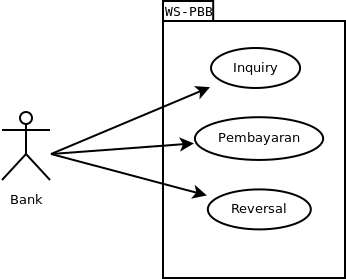
\includegraphics[width=0.5\textwidth]{./resources/uml/uml-use-case}
  \caption{Diagram \textit{use-case}}
  \label{fig:uml-use-case}
\end{figure}

Dari diagram \textit{use-case} diatas, skenarionya adalah bahwa Bank sebagai tempat pembayaran dapat melakukan \textit{request} pada ketiga hal yang disediakan oleh \textit{web services} PBB di DPPK. yaitu :

\begin{itemize}
  \item \textit{Inquiry}
  \item Pembayaran
  \item Reversal
\end{itemize}

Untuk melihat masing-masing proses pada skenario diatas, ada pada diagram \textit{activity} yang dibahas pada bagian selanjutnya. 

\section{Diagram \textit{Activity}}

Diagram \textit{activity} ini akan menunjukan aktivitas yang terjadi untuk setiap skenario pada diagram \textit{use-case}. Berikut skema diagram dari masing-masing skenario yang terbagi menjadi 3 (tiga) diagram berdasarkan jumlah skenario pada diagram \textit{use-case} :

\subsection{Diagram \textit{Activity} Untuk \textit{Inquiry}}

Bagan diagram \textit{activity} untuk \textit{inquiry} ini seperti ditunjukan pada gambar \ref{fig:act-inquiry} :

\begin{figure}[H]
  \centering
  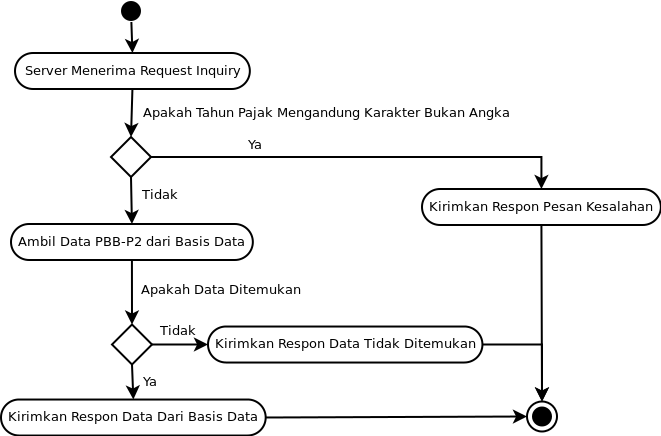
\includegraphics[width=0.8\textwidth]{./resources/uml/uml-act-inquiry}
  \caption{Diagram \textit{Activity} untuk \textit{Inquiry}}
  \label{fig:act-inquiry}
\end{figure}

Aktivitas akan dimulai dari lingkaran penuh di atas, yang kemudian didahului oleh \textit{client} yang melakukan \textit{request} untuk \textit{inquiry} data PBB-P2, hal yang pertama dilakukan adalah melakukan pemeriksaan informasi tahun pajak yang diminta, apakah mengandung karakter atau tidak.

Bila Tahun pajak terisi dengan angka yang wajar, maka aplikasi \textit{web services} akan melakukan koneksi dengan basis data SISMIOP untuk mengambil informasi-informasi yang dibutuhkan oleh \textit{client}.

Bila data tidak ditemukan dalam basis data, maka aplikasi \textit{web services} akan mengirimkan informasi kepada \textit{client} bahwa data yang diminta tidak ditemukan, namun bila data ditemukan, maka disusun dalam format JSON dan dikirimkan ke \textit{client} sebagai respon atas \textit{request} tersebut.

Sampai sini aktivitas selesai.

\subsection{Diagram \textit{Activity} Untuk Pencatatan Pembayaran}

Diagram \textit{activity} untuk melakukan pencatatan pembayaran dapat dilihat seperti pada gambar \ref{fig:act-bayar} :

\begin{figure}[H]
  \centering
  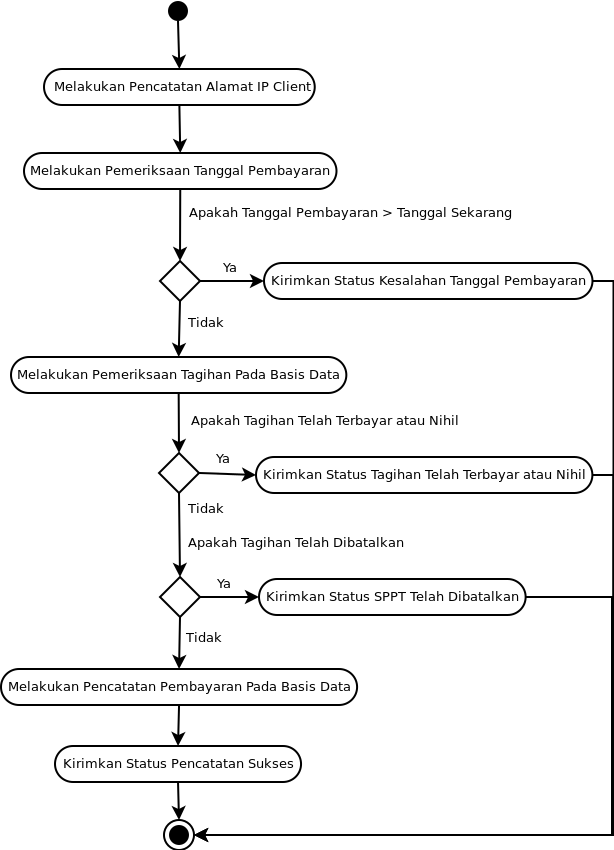
\includegraphics[width=0.8\textwidth]{./resources/uml/uml-act-bayar}
  \caption{Diagram \textit{Activity} Untuk Pencatatan Pembayaran}
  \label{fig:act-bayar}
\end{figure}

Aktivitas pencatatan pembayaran diawali pada saat \textit{client} melakukan \textit{request} pembayaran SPPT PBB-P2, \textit{server web services} akan melakukan pencatatan alamat IP darimana \textit{request} tersebut berasal.

Kemudian \textit{server} akan melakukan pemeriksaan terhadap tanggal pembayaran, apabila tanggal pembayaran melebihi tanggal saat dilakukannya proses pencatatan pembayaran, maka \textit{server} akan mengirimkan status kesalahan tanggal pembayaran ke \textit{client}, dan aktivitas selesai, namun bila tanggal pembayaran kurang dari atau sebelum hari dilakukannya proses pencatatan, maka aktivitas berlanjut ke proses berikutnya.

Pada tahap ini \textit{server} melakukan pemeriksaan tagihan pada basis data, apakah kondisi objek pajak (yang teridentifikasi dari nomor objek pajak) sudah terbayar atau belum, atau tagihannya nihil (tidak ada pajak yang terhutang), bila ya, maka \textit{server} akan mengirimkan status ke \textit{client} bahwa objek yang diminta telah terbayar atau merupakan objek yang piutangnya nihil. bila tidak, maka proses berlanjut.

Proses akhir dari aktivitas ini adalah melakukan pencatatan pembayaran pada basis data, kemudian mengirimkan status bahwa pencatatan tersebut telah selesai. Sampai sini aktivitas telah sampai pada ujung prosesnya.

\subsection{Diagram \textit{Activity} Untuk \textit{Reversal}}

Diagram \textit{activity} untuk melakukan proses \textit{reversal} adalah sebagaimana ditunjukkan pada gambar \ref{fig:act-reversal} :

\begin{figure}[H]
  \centering
  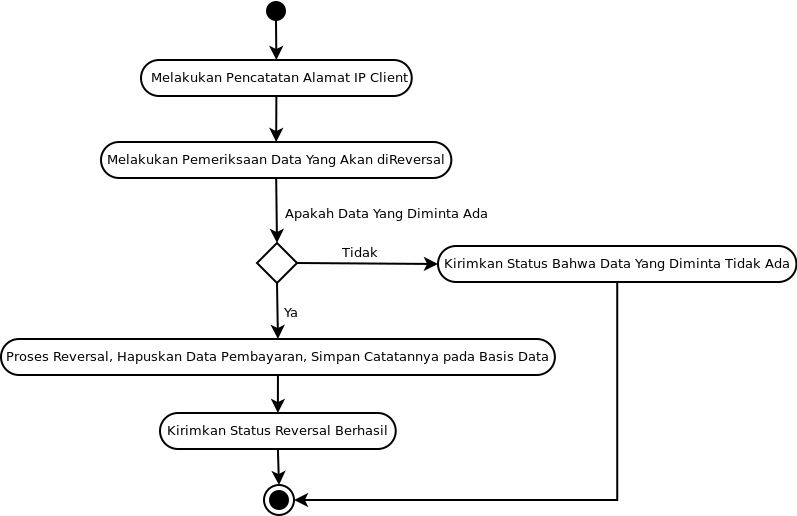
\includegraphics[width=0.8\textwidth]{./resources/uml/uml-act-reversal}
  \caption{Diagram \textit{Activity} Untuk Proses \textit{Reversal}}
  \label{fig:act-reversal}
\end{figure}

Seperti kedua aktivitas sebelumnya, hal yang pertama dilakukan adalah melakukan pencatatan alamat IP dari \textit{client}.

Kemudian melakukan pemeriksan data yang akan direversal, terutama terhadap Nomor Transaksi Pajak Daerah (NTPD) sebagai identitas sebuah transaksi. Apabila data NTPD ini salah, maka \textit{server} akan mengirimkan status kegagalan \textit{reversal} karena data yang diminta tidak ada. Bila data ada, maka melanjutkan ke proses berikutnya.

Langkah berikutnya adalah melakukan pencatatan \textit{request reversal} dan mengirimkan status ke \textit{client} bahwa \textit{reversal} yang diminta telah berhasil dilakukan.

Sampai sini aktivitas \textit{reversal} selesai.

Dari diagram \textit{use-case} dan diagram \textit{activity} telah didapat gambaran umum dari sistem aplikasi yang akan dibangun. Diagram-diagram berikutnya akan lebih detail membahas teknis bagaimana sistem bekerja.

\section{Diagram \textit{Class}}

Pada diagram \textit{class} ini, akan membahas detail dari tiap kelas pembentuk sistem aplikasi \textit{web services} secara keseluruhan. Karena akan menggunakan \textit{framework} Spring yang tentunya memiliki spesifikasi tersendiri, maka untuk memperjelas gambar diagram \textit{class} akan dibagi menjadi beberapa bagian, yaitu :

\begin{enumerate}
  \item Bagian Konfigurasi
  
  Bagian ini adalah kelas-kelas pembentuk konfigurasi \textit{framework} Spring sehingga aplikasi dapat dengan mudah dibangun tanpa perlu memikirkan detail teknis bagaimana Rest harus bekerja. Diagram \textit{class} dari bagian konfigurasi ini seperti ditunjukkan pada gambar \ref{fig:uml-class-konfig} :
  
  \begin{figure}[H]
    \centering
    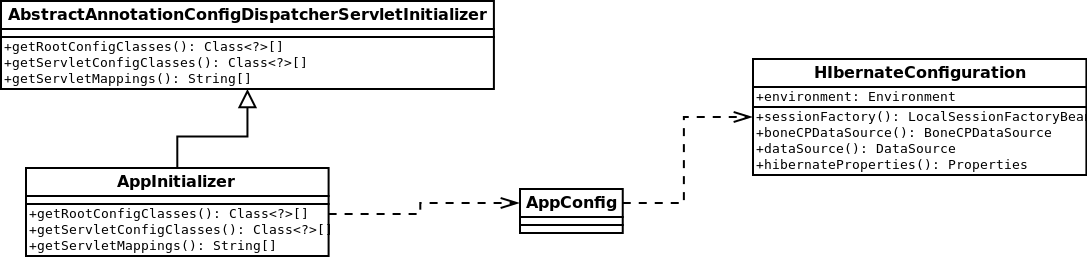
\includegraphics[width=1\textwidth]{./resources/uml/uml-class-konfig}
    \caption{Diagram \textit{Class} Bagian Konfigurasi \textit{Framework} Spring}
    \label{fig:uml-class-konfig}
  \end{figure}
  
  Kelas-kelas inilah yang nantinya mengatur \textit{services} dan konfigurasi koneksi dengan basis data. Awalnya \textit{servlet container} akan memanggil kelas AppInitializer hasil turunan dari kelas atau \textit{interface} AbstractAnnotationConfigDispatcherServletInitializer. Kelas AppInitializer ini membutuhkan kelas AppConfig untuk melakukan Konfigurasi khusus terkait struktur \textit{framework} Spring yang digunakan. Kelas AppConfig ini pun melakukan pemanggilan kelas HibernateConfiguration untuk melakukan konfigurasi komunikasi dengan \textit{server} basis data.
 
  \item Bagian \textit{Inquiry}
  
  Kelas-kelas pada bagian \textit{inquiry} ini, beberapa akan muncul pada bagian transaksi pembayaran ataupun \textit{reversal} karena kelas-kelas tersebut memiliki fungsi yang sama dalam siklus melayani \textit{request} dari \textit{client}. Kelas-kelas pada bagian \textit{inquiry} ini akan terlihat seperti pada gambar \ref{fig:uml-class-inquiry}
  
  \begin{figure}[H]
    \centering
    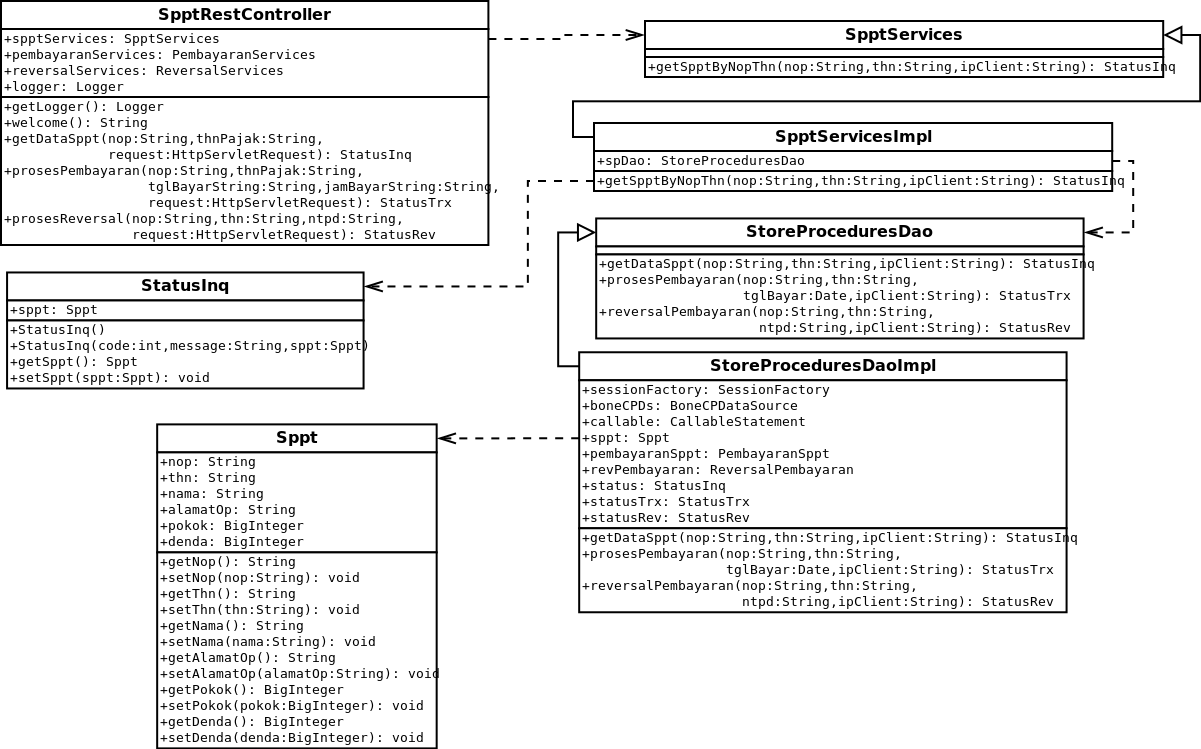
\includegraphics[width=1\textwidth]{./resources/uml/uml-class-inquiry}
    \caption{Diagram \textit{Class} Bagian \textit{Inquiry}}
    \label{fig:uml-class-inquiry}
  \end{figure}
  
  Kelas yang akan menjadi titik awal datangnya sebuah \textit{request} dari \textit{client} adalah kelas SpptRestController, kelas ini yang nantinya akan memilih apakah \textit{request client} adalah \textit{inquiry}, transaksi pembayaran, atau permohonan \textit{reversal}. Kelas SpptRestController ini pula yang nantinya mengirimkan pada \textit{service} yang berkaitan.
  
  Berkaitan dengan bagian \textit{inquiry}, maka begitu ada \textit{request inquiry} dikirimkan oleh \textit{client} dan diterima \textit{server} maka kemudian dipanggil \textit{interface} SpptServices, yang pada struktur kali ini diimplementasikan oleh kelas SpptServicesImpl.
  
  Karena \textit{framework} yang digunakan adalah Spring, maka diperlukan beberapa bagian berdasarkan fungsi utamanya. Fungsi dari masing-masing kelas yang berada pada \textit{framework} Spring yaitu :
  
  \begin{itemize}
    \item \textit{Domain Object}. Kelas-kelas yang memiliki fungsi ini mewakili struktur data persis seperti pada basis data. Penggunaan kelas-kelas pada \textit{domain object} diperlukan karena :
    
    \begin{enumerate}[1)]
      \item Kode program jadi lebih mudah dimengerti dan dipelihara.
      \item Karena Java merupakan bahasa yang \textit{strongly-typed} dan harus di-\textit{compile} terlebih dahulu, akan memudahkan pemeriksaan \textit{bug} pada saat \textit{compile} dibandingkan saat \textit{runtime} atau berjalannya aplikasi.
      \item Memisahkan lapisan data dan antarmuka / \textit{interface}. Apabila ada perubahan skema pada basis data tetapi fitur pada tampilan antarmuka tidak berubah, maka cukup dilakukan perubahan pada lapisan data / \textit{domain object}-nya saja.
      \item Pustaka siap pakai untuk validasi. Di Java, ada pustaka yang berguna untuk melakukan validasi, yaitu JSR-303. Terhadap validasi data yang akan dimasukkan ke dalam basis data, kita tidak perlu melakukan pengecekan seperti contoh kode berikut :
      
      \begin{lstlisting}[language=java]
      if(mydata.getId() == null)
      \end{lstlisting}
      
      Melainkan cukup dengan kode berikut :
      
      \begin{lstlisting}[language=java]
      @NotNull private String Id;
      \end{lstlisting}
    \end{enumerate}
    
    \item \textit{Interface Business Services}
    
    Kelas-kelas pada fungsi ini hanya berupa definisi daftar fitur yang disediakan oleh aplikasi. Seluruh implementasi dikelas ini belum terisi, oleh karena itu dinamakan \textit{interface}. Beberapa alasan penggunaan \textit{interface} atau kelas-kelas abstrak atau tanpa implementasi ini adalah sebagai berikut :
    
    \begin{itemize}
      \item Pada saat membangun sebuah aplikasi \textit{client-server}, maka cukup dengan memberikan kelas-kelas pada \textit{domain object} dan \textit{interface} ini pada \textit{programmer} yang membangun sisi \textit{client}, tanpa perlu menyertakan implementasi dari \textit{interface} yang biasanya cukup besar, aplikasi dapat saling berkomunikasi.
      
      \item Pada saat ada peralihan atau perubahan implementasi perangkat lunak basis data, maka aplikasi disisi \textit{client} tidak perlu berubah.
      
      \item Fitur \textit{declarative transaction} yang dimiliki Spring akan lebih optimal bekerja bila dipisahkan antara \textit{interface} dengan implementasinya.
    \end{itemize}
    
    \item \textit{Implementasi Business Services}
    
    Ini adalah bagian dari implementasi \textit{interface business services}. Jika pada \textit{interface} berisi fitur abstrak, pada bagian ini sudah ada implementasi konkrit untuk masing-masing fitur yang telah didefinisikan pada \textit{interface}. Karena sistem aplikasi akan menggunakan Spring Data JPA, maka diperlukan kelas-kelas lain selain \textit{business services}, yaitu kelas-kelas implementasi \textit{Data Access Object} (DAO).
  \end{itemize}
  
  Implementasi dari kelas SpptServicesImpl akan mengembalikan kelas StatusInq sebagai respon terhadap \textit{request} yang telah sampai ke \textit{server}. Kelas SpptServicesImpl membutuhkan paket kelas DAO berupa \textit{interface} StoreProceduresDao untuk melakukan komunikasi dengan basis data. Implementasi dari \textit{interface} StoreProceduresDao ini adalah kelas StoreProceduresDaoImpl dimana implementasi didalamnya akan menggunakan kelas Sppt untuk menyimpan atau menampung nilai-nilai yang dihasilkan dari pemanggilan \textit{store procedure} pada basis data. Yang pada akhirnya akan dikembalikan kelas Sppt ini dalam bentuk yang terbungkus dalam kelas StatusInq.
  
  \item Bagian Transaksi Pembayaran
  
  Kelas-kelas pembentuk bagian transaksi pembayaran ini adalah kelas-kelas yang saling berhubungan agar \textit{request} transaksi pembayaran dapat diproses sempurna oleh \textit{server}. Kelas-kelas pembentuk bagian transaksi pembayaran ini adalah seperti terlihat pada gambar \ref{fig:uml-class-bayar} :
  
  \begin{figure}[H]
    \centering
    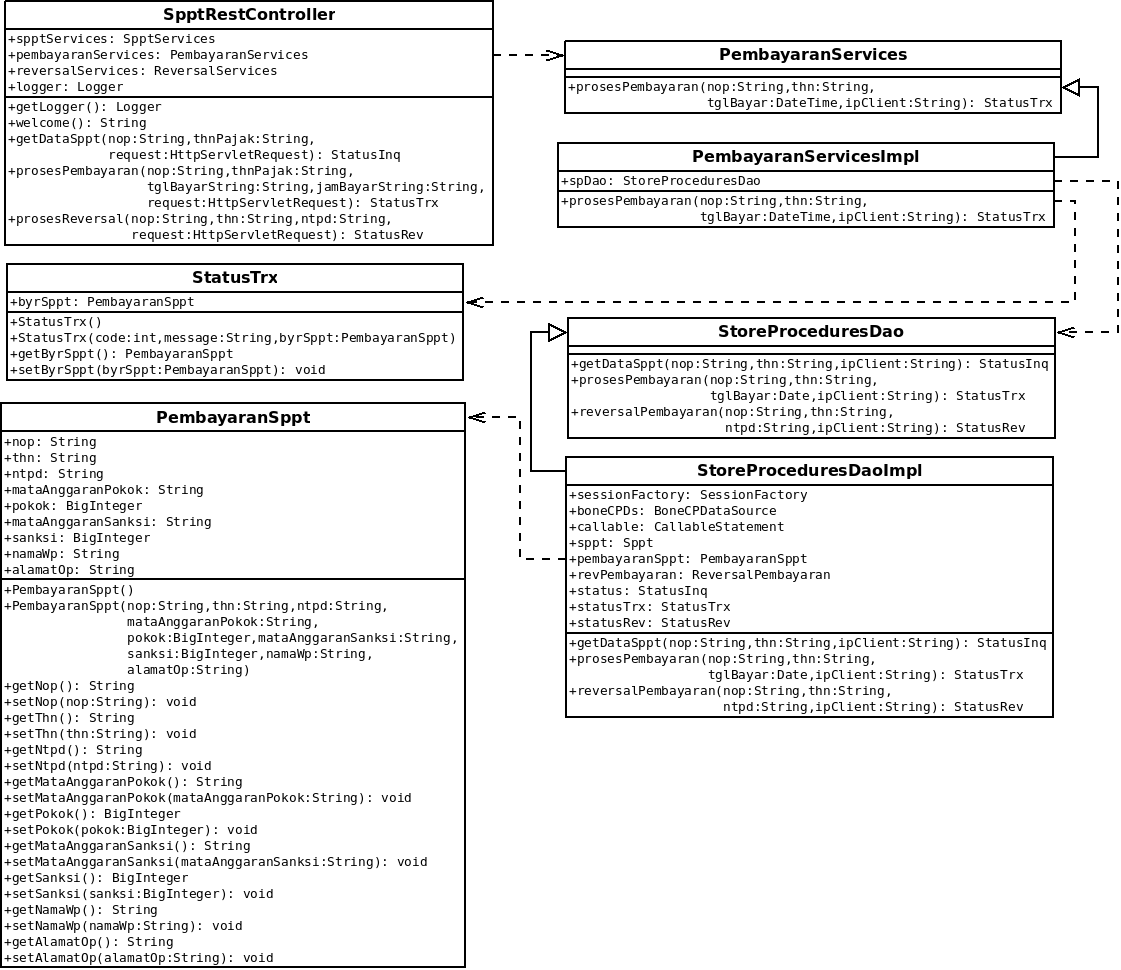
\includegraphics[width=1\textwidth]{./resources/uml/uml-class-bayar}
    \caption{Diagram \textit{Class} Untuk Bagian Pembayaran}
    \label{fig:uml-class-bayar}
  \end{figure}
  
  Seperti bagian sebelumnya, kelas SpptRestController yang sama muncul di bagian ini karena dari kelas inilah titik awal sebuah \textit{request} dari \textit{client} dimulai.
  
  Yang berbeda dari bagian ini adalah kelas-kelas PembayaranServices dan PembayaranServicesImpl sebagai \textit{interface} dan kelas implementasinya yang dibutuhkan oleh \textit{framework} Spring, kemudian ada kelas StatusTrx sebagai pembungkus respon yang nantinya dikirimkan ke \textit{client}, serta kelas PembayaranSppt untuk menampung informasi yang datang dari basis data hasil dari pemanggilan DAO dari kelas StoreProceduresDaoImpl yang sama seperti pada bagian \textit{inquiry}. pada bagian transaksi pembayaran ini pun, kelas PembayaranSppt sebagai bahan respon atas \textit{request} dari \textit{client} akan dibungkus dengan kelas \textit{StatusTrx} agar informasi yang sampai ke \textit{client} dapat lebih jelas.
  
  \item Bagian \textit{Reversal}
  
  Kelas-kelas pembentuk bagian \textit{reversal} ini berfungsi untuk melakukan \textit{reversal} transaksi yang sebelumnya telah terjadi. Kelas-kelas pada bagian ini seperti terlihat pada gambar \ref{fig:uml-class-rev} :
  
  \begin{figure}[H]
    \centering
    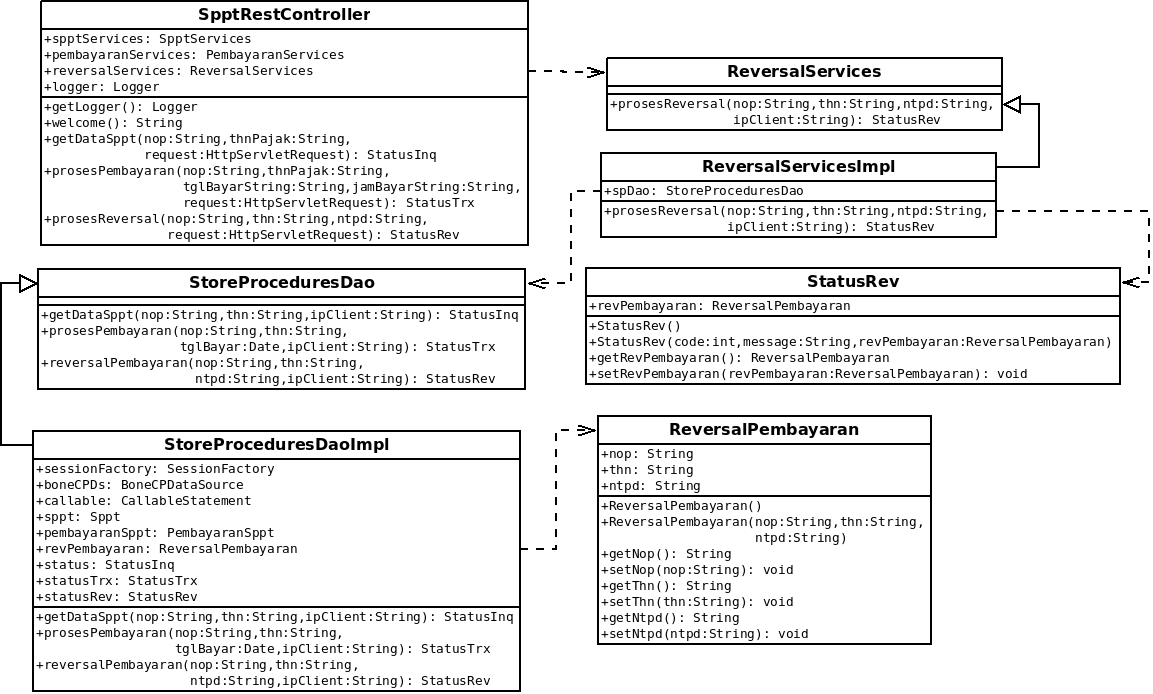
\includegraphics[width=1\textwidth]{./resources/uml/uml-class-rev}
    \caption{Diagram \textit{Class} Yang Berhubungan Dengan Proses \textit{Reversal}}
    \label{fig:uml-class-rev}
  \end{figure}
  
  Seperti pada bagian-bagian sebelumnya, kelas SpptRestController tetap ada sebagai titik awal masuknya sebuah \textit{request} yang akan diproses. Kemudian karena \textit{request} yang diterima berupa proses \textit{reversal} maka akan berhubungan dengan \textit{interface} ReversalServices dan kelas ReversalServicesImpl untuk mengikuti aturan dari \textit{framework} Spring.
  
  Sebagai penghubung komunikasi antara aplikasi dengan basis data, tetap menggunakan \textit{interface} StoreProceduresDao dengan kelas StoreProceduresDaoImpl sebagai implementasinya. Sebagai bahan respon, data-data hasil pengambilan dari basis data akan ditampung pada kelas ReversalPembayaran dengan dibungkus kelas StatusRev untuk mempermudah menambahkan informasi-informasi sukses atau gagalnya operasi yang terjadi pada \textit{server}.
  
\end{enumerate}

\section{Diagram \textit{Sequence}}

Untuk penjelasan diagram \textit{sequence} ini pun, agar diagram terlihat jelas alurnya, maka perlu dipecah menjadi beberapa bagian. Agar lebih mudah memahami prosesnya, diagram akan dipecah seperti pada diagram \textit{class} yaitu hanya saja untuk diagram \textit{sequence} ini akan berbentuk skenario-skenario sebagai berikut :

\subsection{Skenario Konfigurasi \textit{Spring Framework}}

Bagian ini akan menjelaskan bagaimana alur dari awal \textit{server} melakukan inisialisasi sistem, sampai kepada tahap \textit{server} siap menerima \textit{request}. Diagram \textit{sequence} untuk keadaan ini dapat dilihat seperti pada gambar \ref{fig:uml-seq-konf} :
  
  \begin{figure}[H]
    \centering
    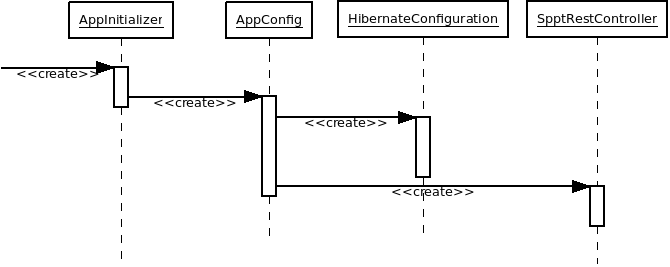
\includegraphics[width=1\textwidth]{./resources/uml/uml-seq-konf}
    \caption{Diagram \textit{Sequence} Untuk Konfigurasi dan Inisialisasi}
    \label{fig:uml-seq-konf}
  \end{figure}
  
  Pada awalnya \textit{servlet container} akan melakukan inisialisasi kelas AppInitializer yang merupakan turunan dari kelas AbstractAnnotationConfigDispatcherServletInitializer, objek AbstractAnnotationConfigDispatcherServletInitializer ini merupakan \textit{interface} yang disediakan \textit{framework} Spring untuk tempat memulai melakukan inisialisasi.
  
  Lalu kelas AppInitializer melakukan inisialisasi terhadap kelas AppConfig untuk melakukan konfigurasi-konfigurasi yang diperlukan agar sistem aplikasi dapat bekerja dengan baik. Salah satu diantaranya adalah melakukan inisialisasi terhadap kelas SpptRestController, kelas inilah yang nantinya melakukan seleksi \textit{request} dan mengirimkan pada kelas \textit{service} yang berkaitan.
  
  Selain melakukan inisialisasi terhadap kelas SpptRestController, kelas AppConfig pun melakukan inisialisasi terhadap kelas HibernateConfiguration. Kelas HibernateConfiguration ini mempersiapkan koneksi dengan basis data dengan menyediakan modul-modul yang dapat digunakan pada sistem aplikasi nantinya.
  
\subsection{Skenario \textit{Inquiry} Gagal Karena Tahun Pajak Bukan Angka}

Skenario ini akan menggambarkan kondisi dimana \textit{client} mengirimkan \textit{request inquiry}, namun setelah diseleksi oleh \textit{server} terdapat karakter bukan angka pada tahun pajak yang di-\textit{request}. Diagram \textit{sequence} dari skenario ini dapat dilihat pada gambar \ref{fig:uml-seq-inq-thn-not-valid} :

\begin{figure}[H]
  \centering
  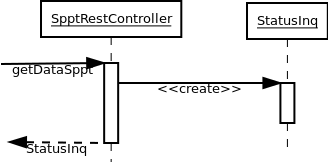
\includegraphics[width=0.8\textwidth]{./resources/uml/uml-seq-inq-thn-not-valid}
  \caption{Diagram \textit{Sequence} Kegagalan \textit{Inquiry} Karena Tahun Pajak Mengandung Karakter Bukan Angka}
  \label{fig:uml-seq-inq-thn-not-valid}
\end{figure}

Objek yang saling berhubungan memang hanya 2 (dua) saja untuk sekenario ini, karena seleksi terhadap karakter pada parameter tahun pajak diperiksa 

\subsection{Skenario \textit{Inquiry} Gagal Karena Data Tidak Ditemukan}

Pada skenario ini, \textit{client} mengirimkan \textit{request} tetapi ada kesalahan bahwa tahun pajak yang di-\textit{request} oleh \textit{client} mengandung karakter bukan angka. Diagram \textit{sequence} dari skenario ini seperti terlihat pada gambar \ref{fig:uml-seq-inq-not-any} :

\begin{figure}[H] 
  \centering
  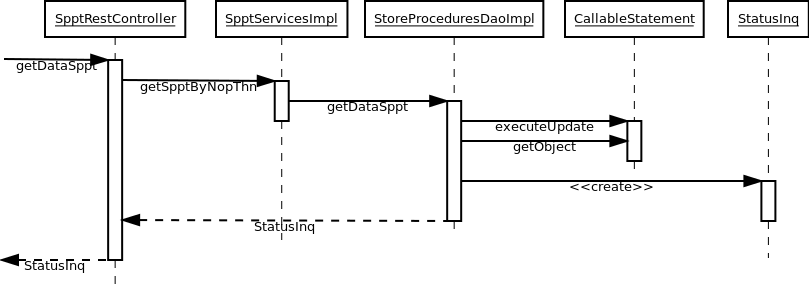
\includegraphics[width=1\textwidth]{./resources/uml/uml-seq-inq-not-any}
  \caption{Diagram \textit{Sequence} Kegagal \textit{Inquiry} Karena Data Tidak Ada Dalam Basis Data}
  \label{fig:uml-seq-inq-not-any}
\end{figure}

Pada diagram \textit{sequence} tersebut, permintaan atau \textit{request} dari \textit{client} akan diterima \textit{server} dan diteruskan oleh \textit{framework} Spring ke \textit{method} getDataSppt milik kelas SpptRestController.

Kemudian \textit{method} getDataSppt akan memanggil \textit{method} getSpptByNopThn milik kelas SpptServicesImpl, yang didalamnya hanya memanggil \textit{method} getDataSppt milik kelas StoreProceduresDaoImpl.

Didalam \textit{method} getDataSppt milik kelas StoreProceduresDaoImpl, terdapat proses koneksi ke basis data melalui kelas CallableStatement, yang pertama melakukan pemanggilan \textit{method} executeUpdate milik untuk mengeksekusi atau memanggil \textit{store procedure} milik basis data, kemudian mengambil nilai balikkannya melalui \textit{method} getObject.

Terakhir adalah melakukan pemeriksaan terhadap nilai balikan dari pembanggil \textit{store procedure} milik basis data, bila nilai kembalian nihil, maka \textit{method} getDataSppt akan membuat instan dari kelas StatusInq, kemudian nilainya dikembalikan ke kelas SpptRestController yang tentu saja dikirimkan hasilnya ke \textit{client}.

\subsection{Skenario \textit{Inquiry} Gagal Karena Kesalahan Server}

Pada skenario ini, \textit{client} melakukan \textit{request inquiry} ke \textit{server}, namun karena beberapa hal, komunikasi antara \textit{server} basis data dan \textit{server} aplikasi mengalami gangguan, sehingga proses \textit{inquiry} gagal dan mengirimkan pesan ke \textit{client} bahwa \textit{request} yang dikirimkan telah gagal diproses. Gambar Diagram \textit{sequence} dari skenario ini dapat dilihat seperti pada gambar \ref{fig:uml-seq-inq-db-error} :

\begin{figure}[H]
  \centering
  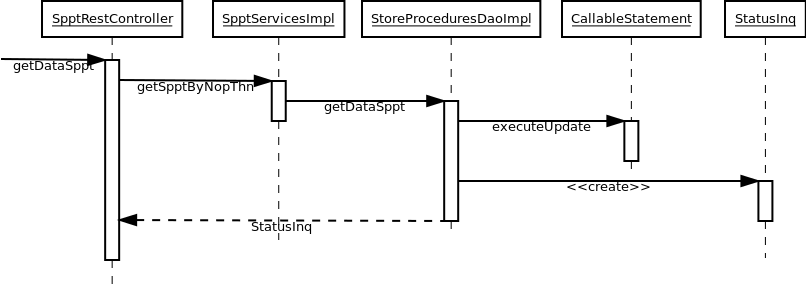
\includegraphics[width=1\textwidth]{./resources/uml/uml-seq-inq-db-error}
  \caption{Diagram \textit{Sequence} Untuk Proses \textit{Inquiry} Yang Gagal Karena Kesalahan Server}
  \label{fig:uml-seq-inq-db-error}
\end{figure}

Diagramnya terlihat sama dengan skenario sebelumnya, yaitu \textit{inquiry} yang gagal karena datanya tidak ada, yang membedakan adalah pada saat \textit{method} getDataSppt milik kelas StoreProceduresDaoImpl melakukan pemanggilan \textit{store procedure} milik basis data melalui \textit{method} executeUpdate pada kelas CallableStatement ada kesalahan, sehingga \textit{method} getDataSppt milik kelas StoreProceduresDaoImpl membuat instan dari kelas StatusInq dan mengembalikannya ke kelas SpptRestController yang kemudian menjadi respon yang dikirim ke \textit{client} sebagai informasi bahwa \textit{request} yang dikirimkan ke \textit{server} gagal diproses.

\subsection{Skenario \textit{Inquiry} Sukses}

Untuk alur proses \textit{inquiry} yang sukses, diagram \textit{sequence}-nya dapat dilihat seperti pada gambar \ref{fig:uml-seq-inq} :
  
  \begin{figure}[H]
    \centering
    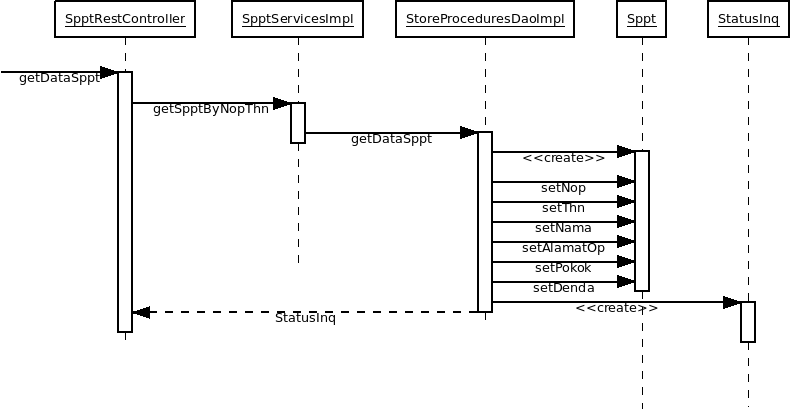
\includegraphics[width=1\textwidth]{./resources/uml/uml-seq-inquiry}
    \caption{Diagram \textit{Sequence} Untuk Menangani \textit{Request Inquiry}}
    \label{fig:uml-seq-inq}
  \end{figure}
  
  Seperti awal dari setiap proses \textit{request} Rest, pada fungsi \textit{inquiry} ini pun berawal dari kelas SpptRestController. Kelas SpptRestController ini kemudian menyalurkannya ke kelas SpptServicesImpl dengan memanggil \textit{method} getSpptByNopThn. Di dalam \textit{method} getSpptByNopThn, kelas SpptServicesImpl memanggil \textit{method} getDataSppt milik kelas StoreProceduresDaoImpl.
  
  Pada kelas StoreProceduresDaoImpl, \textit{method} getDataSppt melakukan koneksi ke basis data dan menampung hasilnya pada kelas Sppt. Hasil-hasil yang diperoleh dari basis data berupa NOP, Tahun Pajak, Nama Wajib Pajak, Alamat Objek Pajak, Besarnya tagihan pokok, dan besarnya Denda Administrasi. Semuanya ditampung yang ditandai dengan pemanggilan \textit{method} setNop, setThn, setNama, setAlamatOp, setPokok, dan setDenda.
  
  Sebelum dikirimkan kembali ke \textit{client}, maka data atau informasi yang ditampung dalam kelas Sppt dipaketkan dengan kelas StatusInq, yang hasilnya dikembalikan ke \textit{client} dalam bentuk kelas StatusInq.

\subsection{Skenario Transaksi Pembayaran Gagal Karena Jam Pembayaran Melebihi Jam Pencatatan}
\subsection{Skenario Transaksi Pembayaran Gagal Karena Tagihan Telah Terbayar Atau Nihil}
\subsection{Skenario Transaksi Pembayaran Gagal Karena Telah Dibatalkan}
\subsection{Skenario Transaksi Pembayaran Gagal Karena Kesalahan Server}
\subsection{Skenario Transaksi Pembayaran Sukses}
\subsection{Skenario \textit{Reversal} Gagal Karena Data Yang Diminta Tidak Ada}
\subsection{Skenario \textit{Reversal} Gagal Karena Ada Data Pembayaran Yang Tercatat Ganda}
\subsection{Skenario \textit{Reversal} Gagal Karena Kesalahan Server}
\subsection{Skenario \textit{Reversal} Sukses}

\begin{enumerate}
  
  
  \item Bagian \textit{Inquiry}
  
  
  
  \item Bagian Transaksi Pembayaran
  
  Pada bagian-bagian yang menangani transaksi pembayaran, objek-objek yang berhubungan akan terlihat berkomunikasi pada diagram \textit{sequence} seperti pada gambar \ref{fig:uml-seq-trx} :
  
  \begin{figure}[H]
    \centering
    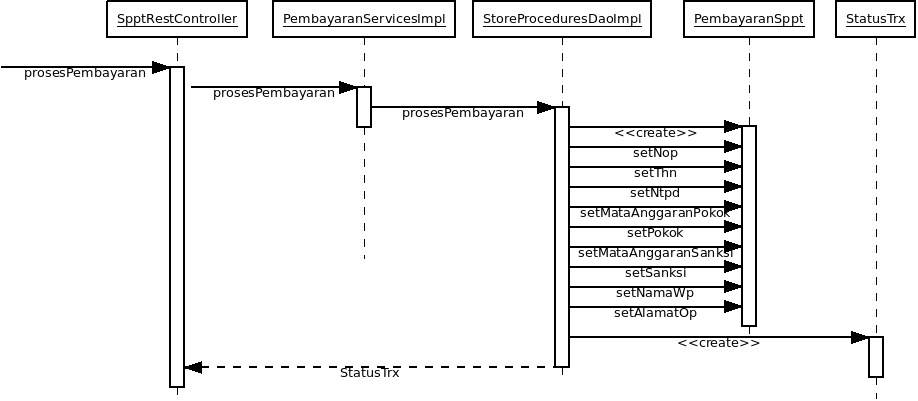
\includegraphics[width=1\textwidth]{./resources/uml/uml-seq-trx}
    \caption{Diagram \textit{Sequence} Untuk Proses Pencatatan Transaksi Pembayaran}
    \label{fig:uml-seq-trx}
  \end{figure}
  
  Seperti proses pada \textit{request inquiry}, pada proses pencatatan pembayaran, \textit{request} akan diterima dan disaring pada kelas SpptRestController. Karena \textit{request}-nya adalah melakukan pencatatan pembayaran, maka yang dipanggil adalah \textit{method} prosesPembayaran milik kelas SpptRestController.
  
  Dari \textit{method} prosesPembayaran milik kelas SpptRestController, didalamnya memanggil \textit{method} dengan nama yang sama, yaitu \textit{method} prosesPembayaran tetapi milik kelas PembayaranServicesImpl. 
  
  Dari \textit{method} prosesPembayaran milik kelas PembayaranServicesImpl pada lapisan \textit{services}, kemudian memanggil \textit{method} dengan nama yang sama pula, yaitu \textit{method} prosesPembayaran, tetapi kali ini milik kelas StoreProceduresDaoImpl sebagai lapisan penghubung antara aplikasi dengan basis data.
  
  Pada \textit{method} prosesPembayaran milik kelas StoreProceduresDaoImpl ini, proses didalamnya adalah memanggil \textit{store procedure} milik basis data Oracle, yang kemudian, hasil pencatatan akan ditampung dalam kelas PembayaranSppt.
  
  \textit{Method} prosesPembayaran milik kelas StoreProceduresDaoImpl akhirnya akan membungkus kelas PembayaranSppt yang sudah menampung beberapa parameter pencatatan pembayaran di dalam kelas StatusTrx, dan mengembalikan kelas StatusTrx ke kelas SpptRestController untuk dijadikan respon terhadap \textit{request} yang telah diterima dari \textit{client}.
  
  \item Bagian \textit{Reversal}
  
  Pada fungsi \textit{reversal}, diagram \textit{sequence} yang terlihat akan mirip dengan diagram pada fungsi transaksi pembayaran atau \textit{request inquiry}, seperti terlihat pada gambar \ref{fig:uml-seq-rev} :
  
  \begin{figure}[H]
    \centering
    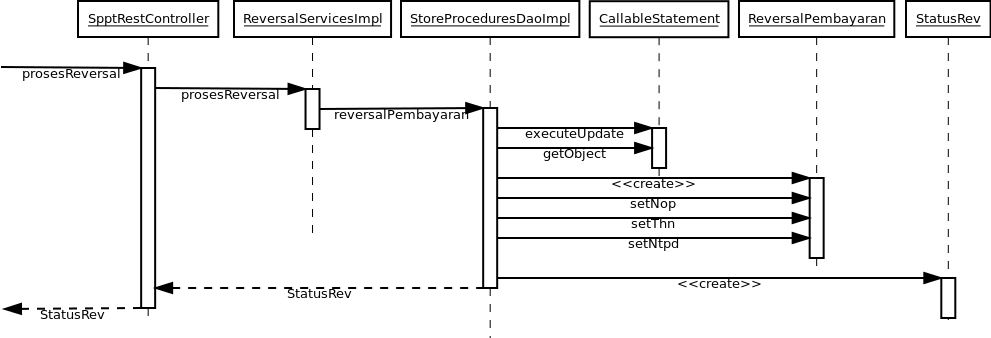
\includegraphics[width=1\textwidth]{./resources/uml/uml-seq-rev}
    \caption{Diagram \textit{Sequence} Untuk Fungsi \textit{Reversal}}
    \label{fig:uml-seq-rev}
  \end{figure}
  
  Seperti beberapa \textit{request} sebelumnya, \textit{request reversal} pun akan dimulai dari kelas SpptRestController pada \textit{method} prosesReversal.
  
  Pada \textit{method} prosesReversal kelas SpptRestController akan memanggil \textit{method} yang sama namanya, yaitu \textit{method} prosesReversal tetapi milik kelas ReversalServicesImpl.
  
  Dari \textit{method} prosesReversal milik kelas ReversalServicesImpl ini, kemudian akan memanggil \textit{method} reversalPembayaran pada kelas StoreProceduresImpl yang didalamnya memuat koneksi ke basis data kemudian memanggil \textit{store procedure} yang ada pada basis data dan menampung hasilnya pada kelas ReversalPembayaran.
  
  Pada langkah terakhir, \textit{method} reversalPembayaran kelas StoreProceduresImpl ini akan membungkus kelas ReversalPembayaran di dalam kelas StatusRev yang dikembalikan ke kelas SpptRestController agar dijadikan bahan respon terhadap \textit{request} yang dilakukan oleh \textit{client}.
\end{enumerate}

\chapter{DESKRIPSI SUB SISTEM}

Karena sistem yang akan dibuat menggunakan desain berorientasi objek, maka penjelasan lebih detail dari sub-sistem ini akan lebih mudah bila kita melihat diagram \textit{class} yang telah dijelaskan dan digambarkan pada bagian sebelumnya, namun kali ini akan dijelaskan lebih detail.

\section{Kelas AppInitializer}

Kelas ini menjadi kelas pembuka bagi sistem aplikasi yang menggunakan \textit{framework} Spring karena kelas ini mengimplementasikan \textit{interface} dari \textit{framework} Spring yang bernama AbstractAnnotationConfigDispatcherServletInitializer.

Diagram dari kelas AppInitializer ini seperti ditunjukkan pada gambar \ref{fig:uml-class-AppInitializer} :

\begin{figure}[H]
  \centering
  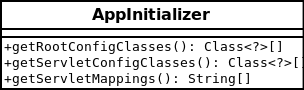
\includegraphics[width=0.5\textwidth]{./resources/uml/uml-class-AppInitializer}
  \caption{Diagram Kelas AppInitializer}
  \label{fig:uml-class-AppInitializer}
\end{figure}

Karena kelas ini adalah implementasi dari \textit{interface} AbstractAnnotationConfigDispatcherServletInitializer, maka harus mengimplementasikan pula ketiga \textit{method} yang ada pada \textit{interface} tersebut, yaitu \textit{method} getRootConfigClasses, \textit{method} getServletConfigClasses, dan \textit{method} getServletMappings.

\section{Kelas AppConfig}

Kelas ini merupakan kelas konfigurasi yang digunakan \textit{framework} Spring untuk melakukan konfigurasi terhadap sistem aplikasi yang akan dijalankan. Bukan karena mengimplementasikan kelas atau \textit{interface} yang dibawa oleh Spring, melainkan karena dideklarasikan sebagai kelas yang menangani konfigurasi sistem aplikasi di kelas AppInitializer.

Pada kelas ini, karena menggunakan fitur MVC (\textit{Model-View-Controller}) dari Spring, maka akan ada beberapa kelas yang ditujukan untuk fungsinya masing-masing, dikelas inilah nantinya kelas-kelas tersebut dideklarasikan, pada kelas ini pula disebutkan kelas yang bertanggung jawab untuk melakukan konfigurasi-konfigurasi yang lain termasuk konfigurasi komunikasi dengan sistem basis data.

Diagram dari kelas AppConfig ini seperti ditampilkan pada gambar \ref{fig:uml-class-AppConfig} :

\begin{figure}[H]
  \centering
  
\includegraphics[width=0.3\textwidth]{./resources/uml/uml-class-AppConfig}
  \caption{Diagram Kelas AppConfig}
  \label{fig:uml-class-AppConfig}
\end{figure}

Kelas ini memang terlihat kosong, karena konfigurasi-konfigurasi yang dilakukan nantinya akan menggunakan fitur \textit{annotation} milik Java agar memudahkan pembacaan kode dan menyederhanakan konfigurasi.

\section{Kelas HibernateConfiguration}

Kelas ini bertugas melakukan konfigurasi komunikasi dengan sistem basis data. Diagram dari kelas HibernateConfiguration ini seperti terlihat pada gambar \ref{fig:uml-class-HibernateConfiguration} :

\begin{figure}[H]
  \centering
  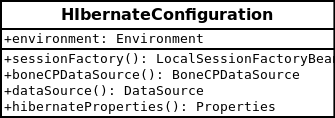
\includegraphics[width=0.8\textwidth]{./resources/uml/uml-class-HibernateConfiguration}
  \caption{Diagram Kelas HibernateConfiguration}
  \label{fig:uml-class-HibernateConfiguration}
\end{figure}

Kelas ini terdiri dari 1 (satu) properti dan 4 (empat) \textit{method}. Propertinya diberi nama environment, karena properti ini akan bertugas menampung nilai-nilai konfigurasi standar yang berada pada \textit{file} yang terpisah.

\textit{Method} yang pertama adalah \textit{method} sessionFactory. \textit{Method} sessionFactory ini akan bertugas mengembalikan nilai sebuah kelas LocalSessionFactoryBean dimana kelas ini yang menjadi sesi dari tiap \textit{user} untuk melakukan koneksi ke basis data nantinya. Untuk menyediakan akses data yang cepat dan optimal, \textit{method} ini akan menggunakan \textit{connection pool} milik BoneCP.

\textit{Method} berikutnya adalah boneCPDataSource, \textit{method} ini akan menyediakan konfigurasi untuk melakukan koneksi ke basis data sebagai sumber data, yang dikembalikan dalam bentuk kelas BoneCPDataSource. \textit{Method} ini menjadi sumber untuk pengambilan data apapun pada basis data dengan menggunakan \textit{connection pool} BoneCP.

\textit{Method} dataSource adalah \textit{method} standar yang menggunakan \textit{connection pool} yang dibawa oleh Hibernate yang digunakan untuk melakukan pemeriksaan awal koneksi ke basis data, apabila menggunakan \textit{method} ini berhasil, maka tidak akan menjadi masalah apabila dilakukan menggunakan \textit{connection pool} yang lain.

\textit{Method} yang terakhir adalah hibernateProperties, \textit{method} ini melakukan konfigurasi terhadap Hibernate yang nantinya digunakan pada \textit{method} sessionFactory.

\section{Kelas SpptRestController}

Kelas ini yang menjadi gerbang pertama yang menentukan kemana sebuah \textit{request} akan di respon. Diagram kelas dari SpptRestController ini akan terlihat seperti pada gambar \ref{fig:uml-class-SpptRestController} :

\begin{figure}[H]
  \centering
  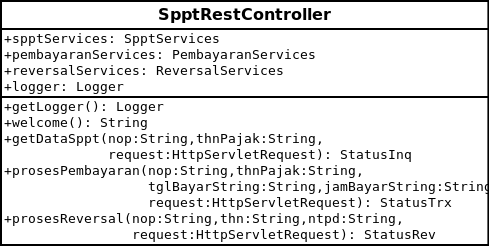
\includegraphics[width=0.8\textwidth]{./resources/uml/uml-class-SpptRestController}
  \caption{Diagram Kelas SpptRestController}
  \label{fig:uml-class-SpptRestController}
\end{figure}

Kelas ini memiliki 4 (empat) properti dan 5 (lima) \textit{method}. Penjelasan dan fungsi masing-masing properti dan \textit{method} tersebut yaitu sebagai berikut :

\begin{itemize}
  \item Properti
  
  \begin{itemize}
    \item Properti spptServices
    
    Properti ini yang akan mengatur layanan yang menangani permintaan / \textit{request inquiry} dari \textit{client}.
    
    \item Properti pembayaranServices
    
    Properti pembayaranServices ini akan mengatur layanan yang menangani permintaan / \textit{request} pencatatan pembayaran dari \textit{client}.
    
    \item Properti reversalServices
    
    Properti reversalServices ini akan mengatur layanan yang menangani permintaan / \textit{request reversal} dari \textit{client} karena ada kesalahan pencatatan pembayaran sebelumnya.
    
    \item Properti logger
    
    Properti logger digunakan untuk melakukan pencatatan aktifitas sistem aplikasi ke dalam sebuah \textit{file} pada saat sistem aplikasi berjalan dan digunakan. Kondisi ini diperlukan agar memudahkan diagnosa sistem apabila terjadi anomali-anomali proses yang tidak diinginkan.
   
  \end{itemize}
  
  \item \textit{Method}
  
  \begin{itemize}
    \item \textit{Method} getLogger
    
    \textit{Method} getLogger ini menyediakan akses ke properti logger agar dapat mencatat kejadian saat \textit{runtime} dari kelas mana pun pada sistem aplikasi.
    
    \item \textit{Method} welcome
    
    \textit{Method} welcome ini adalah halaman muka dari layanan Rest, jadi setiap \textit{request} yang dilayangkan ke \textit{root slash} ("/"), maka akan direspon oleh \textit{method} welcome ini.
    
    \item \textit{Method} getDataSppt
    
    \textit{Method} getDataSppt difungsikan sebagai tempat masuknya \textit{request inquiry} data tagihan SPPT PBB-P2, nantinya \textit{method} ini akan mengembalikan respon dalam bentuk kelas StatusInq yang telah diubah dalam format JSON.
    
    \item \textit{Method} prosesPembayaran
    
    \textit{Method} prosesPembayaran ini akan bertugas menangani \textit{request} pencatatan pembayaran dari \textit{client}. \textit{Method} ini akan mengembalikan kelas StatusTrx yang tentunya telah diubah dalam format JSON.
    
    \item \textit{Method} prosesReversal
    
    \textit{Method} prosesReversal ini seperti \textit{method} getDataSppt dan \textit{method} prosesPembayaran yang menangani sebuah \textit{request} dari \textit{client}, namun \textit{method} prosesReversal ini akan menangani \textit{request reversal} dari pembayaran yang telah tercatat dalam basis data.
    
    Penyebab proses \textit{reversal} ini karena adanya kesalahan pencatatan pembayaran yang sebelumnya terjadi, misalkan pada saat \textit{client} melakukan \textit{request} pencatatan pembayaran, sebelum \textit{client} mendapatkan respon dari \textit{server} koneksi tiba-tiba terputus dan \textit{client} tidak pernah mendapatkan respon atas \textit{request}-nya, maka untuk memastikan adalah melakukan \textit{request reversal} dan melakukan \textit{request} pencatatan pembayaran kembali.
    
  \end{itemize}
\end{itemize}

\section{Kelas SpptServicesImpl}

Kelas SpptServicesImpl akan melayani \textit{request inquiry} dan melanjutkannya ke kelas-kelas yang menangani basis data. Diagram kelas dari SpptServicesImpl ini adalah seperti pada gambar \ref{fig:uml-class-SpptServicesImpl}

\begin{figure}[H]
  \centering
  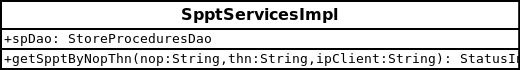
\includegraphics[width=1\textwidth]{./resources/uml/uml-class-SpptServicesImpl}
  \caption{Diagram Kelas SpptServicesImpl}
  \label{fig:uml-class-SpptServicesImpl}
\end{figure}

Kelas SpptServicesImpl ini memiliki 1 (satu) properti dan 1 (satu) \textit{method}. Propertinya bernama spDao, untuk menampung kelas StoreProceduresDao yang menangani semua hal mengenai eksekusi \textit{store procedure} pada basis data.

\textit{Method} dari kelas ini bernama getSpptByNopThn yang berfungsi melakukan pemanggilan terhadap kelas yang bertugas menghubungi basis data yang pencarian datanya berdasarkan Nomor Objek Pajak (NOP) dan tahun pajak.

\section{Kelas PembayaranServicesImpl}

Kelas PembayaranServicesImpl bertugas melayani permintaan terhadap pencatatan pembayaran yang posisinya berada di tengah dan menjadi penghubung antara \textit{interface} dengan kelas-kelas \textit{data access}. Diagram kelas PembayaranServicesImpl ini seperti pada gambar \ref{fig:uml-class-PembayaranServicesImpl} :

\begin{figure}[H]
  \centering
  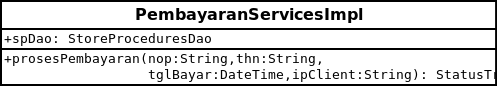
\includegraphics[width=1\textwidth]{./resources/uml/uml-class-PembayaranServicesImpl}
  \caption{Diagram Kelas PembayaranServicesImpl}
  \label{fig:uml-class-PembayaranServicesImpl}
\end{figure}

Kelas ini memiliki 1 (satu) properti dan 1 (satu) \textit{method}, properti yang dimiliki bernama spDao, ini adalah instan dari kelas atau \textit{interface} StoreProceduresDao yang bertugas melakukan komunikasi dengan sistem aplikasi basis data.

Sedangkan \textit{method} prosesPembayaran adalah \textit{method} yang bertugas sebagai penghubung antara \textit{interface} dalam hal ini kelas SpptRestController, dengan kelas yang berhubungan dan berkomunikasi langsung dengan basis data untuk melakukan eksekusi pencatatan pembayaran.

\section{Kelas ReversalServicesImpl}

Seperti kelas PembayaranServicesImpl dan SpptServicesImpl, kelas ReversalServicesImpl bertugas menjadi penghubung antara \textit{interface} yang menangani proses \textit{reversal} dengan kelas-kelas yang berhubungan dengan basis data. 

Diagram kelas ReversalServicesImpl ini seperti terlihat pada gambar \ref{fig:uml-class-ReversalServicesImpl} :

\begin{figure}[H]
  \centering
  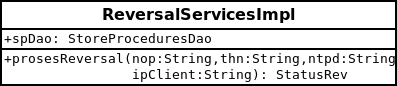
\includegraphics[width=0.5\textwidth]{./resources/uml/uml-class-ReversalServicesImpl}
  \caption{Diagram Kelas ReversalServicesImpl}
  \label{fig:uml-class-ReversalServicesImpl}
\end{figure}

Seperti terlihat pada diagram bahwa kelas ReversalServicesImpl ini memiliki sebuah properti dan sebuah \textit{method}.

Properti yang dimiliki kelas ReversalServicesImpl ini bernama spDao yang merupakan instan dari kelas StoreProceduresDao, dengan \textit{method} bernama prosesReversal, \textit{method} ini nantinya akan berkomunikasi dengan kelas StoreProceduresDao melalui instan kelas spDao yang menjadi penghubung dengan sistem aplikasi basis data.

\section{Kelas StoreProceduresDaoImpl}

Kelas StoreProceduresDaoImpl ini yang mengimplementasikan \textit{interface} StoreProceduresDao yang fungsinya melakukan komunikasi dengan sistem basis data. Diagram kelas StoreProceduresDaoImpl ini seperti terlihat pada gambar \ref{fig:uml-class-StoreProceduresDaoImpl} :

\begin{figure}[H]
  \centering
  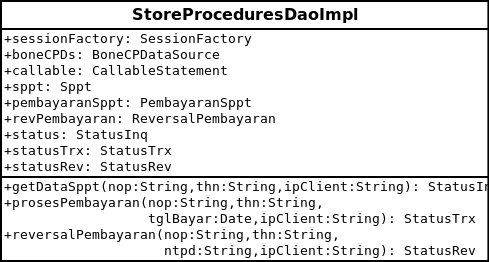
\includegraphics[width=0.8\textwidth]{./resources/uml/uml-class-StoreProceduresDaoImpl}
  \caption{Diagram Kelas StoreProceduresDaoImpl}
  \label{fig:uml-class-StoreProceduresDaoImpl}
\end{figure}

Kelas ini memiliki beberapa properti dan 3 (tiga) buah \textit{method}. Properti yang pertama bernama sessionFactory, ini adalah instan dari kelas SessionFactory yang bertugas membuka sesi komunikasi dengan sistem basis data.

Properti yang kedua adalah boneCPDs, yang merupakan instan dari kelas BoneCPDataSource. Properti ini akan melaksanakan tugasnya dengan \textit{framework} Hibernate menggunakan \textit{connection pool} dari BoneCP untuk hasil komunikasi yang lebih optimal.

Properti yang ketiga adalah callable yang merupakan instan dari kelas CallableStatement, properti ini akan menyediakan perangkat komunikasi yang mampu melakukan eksekusi terhadap \textit{store procedure} yang berada pada basis data.

Properti selanjutnya adalah sppt, pembayaranSppt, dan revPembayaran yang secara berurutan adalah instan dari kelas Sppt, PembayaranSppt, dan ReversalPembayaran. Ketiga properti ini memiliki fungsi yang sama, yaitu menampung nilai yang dikembalikan saat melakukan eksekusi \textit{store procedure} dari sistem basis data.

Properti berikutnya yaitu status, statusTrx, dan statusRev, yang secara berurutan merupakan instan dari kelas StatusInq, StatusTrx, dan StatusRev. Fungsi dari ketiga properti ini yaitu sebagai pembungkus, atau penjelas informasi terhadap respon dari \textit{request} yang dikirimkan oleh \textit{client}.

Untuk \textit{method} yang pertama adalah \textit{method} getDataSppt, yang fungsinya melakukan komunikasi dengan sistem basis data untuk memberikan respon terhadap \textit{request inquiry} dari \textit{client}.

\textit{Method} yang kedua adalah \textit{method} prosesPembayaran, yang fungsinya melakukan komunikasi dengan sistem basis data untuk memberikan respon terhadap \textit{request} pencatatan pembayaran di \textit{client}.

Sedangkan \textit{method} reversalPembayaran berfungsi melakukan komunikasi dengan sistem basis data untuk memberikan respon terhadap \textit{request reversal} pembayaran dari \textit{client}.

\section{Kelas StatusInq}

Kelas StatusInq ini digunakan untuk membungkus data respon sebuah \textit{inquiry} menjadi informasi yang lebih jelas karena ada penjelasan status respon yang diberikan. Misalkan, data \textit{inquiry} tidak muncul, maka kelas ini akan memberikan informasi lain apakah nomor objek pajak yang diminta ada atau tidak, atau kondisi nomor objek pajak tidak muncul karena telah terbayarkan.

Diagram kelas StatusInq ini seperti terlihat pada gambar \ref{fig:uml-class-StatusInq} :

\begin{figure}[H]
  \centering
  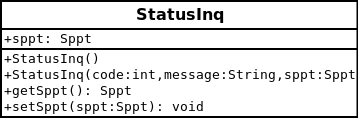
\includegraphics[width=0.5\textwidth]{./resources/uml/uml-class-StatusInq}
  \caption{Diagram Kelas StatusInq}
  \label{fig:uml-class-StatusInq}
\end{figure}

Kelas ini hanya memiliki 1 (satu) properti, 2 (dua) konstruktor, dan 2 (dua) \textit{method}.

Properti pada kelas ini diberi nama sppt yang merupakan instan dari kelas Sppt. Seperti dijelaskan pada bagian sebelumnya, kelas Sppt ini digunakan untuk menampung nilai yang dikembalikan oleh sistem basis data pada saat pemanggilan \textit{store procedure inquiry}.

Kontruktor disediakan 2 (dua), untuk menjadikan kelas ini fleksibel dalam implementasi instan. Sedangkan 2 (dua) \textit{method} yang disediakan sebetulnya untuk melakukan akses \textit{set} dan \textit{get} terhadap properti sppt.

\section{Kelas StatusTrx}

Kelas StatusTrx ini berfungsi membungkus informasi pencatatan transaksi pembayaran agar respon kepada \textit{client} lebih jelas. Diagram kelas dari kelas StatusTrx ini seperti terlihat pada gambar \ref{fig:uml-class-StatusTrx} :

\begin{figure}[H]
  \centering
  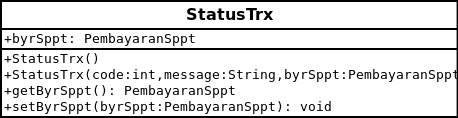
\includegraphics[width=0.5\textwidth]{./resources/uml/uml-class-StatusTrx}
  \caption{Diagram Kelas StatusTrx}
  \label{fig:uml-class-StatusTrx}
\end{figure}

Seperti kelas StatusInq, kelas ini pun memiliki sebuah properti, 2 (dua) buah kontruktor, dan 2 (dua) buah \textit{method}.

Properti pada kelas ini bernama byrSppt yang merupakan instan dari kelas PembayaranSppt, yang fungsinya adalah menampung hasil respon dari sistem basis data atas eksekusi \textit{store procedure} untuk pencatatan pembayaran.

Fungsi dari 2 (dua) kontruktor yang ada pada kelas ini pun ditujukan agar pembentukan instan agar lebih fleksibel. Kedua \textit{method} pun dimaksudkan untuk memberikan akses pada properti dari kelas ini.

\section{Kelas StatusRev}

Kelas StatusRev ini berfungsi untuk membungkus informasi \textit{reversal} agar respon terhadap \textit{request client} lebih jelas. Diagram kelas StatusRev ini dapat dilihat pada gambar \ref{fig:uml-class-StatusRev} :

\begin{figure}[H]
  \centering
  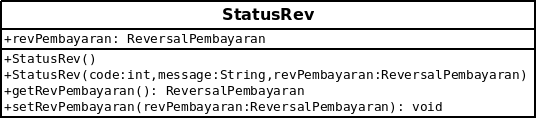
\includegraphics[width=0.8\textwidth]{./resources/uml/uml-class-StatusRev}
  \caption{Diagram Kelas StatusRev}
  \label{fig:uml-class-StatusRev}
\end{figure}

Seperti kelas StatusInq dan StatusTrx, kelas ini pun terdiri dari sebuah properti, 2 (dua) buah konstruktor, dan 2 (dua) buah \textit{method}. 

Properti kelas ini bernama revPembayaran yang merupakan instan dari kelas ReversalPembayaran, yang fungsinya menampung hasil respon dari basis data terhadap eksekusi \textit{store procedure reversal} pembayaran.

Kedua konstruktor yang disediakan untuk menjadikan pembuatan instan kelas ini lebih fleksibel, sedangkan dua \textit{method} yang disediakan merupakan fasilitas untuk melakukan akses terhadap properti kelas ini.

\section{Kelas Sppt}

Kelas Sppt ini adalah kelas yang menampung hasil respon dari pemanggilan atau eksekusi \textit{store procedure inquiry} yang ada pada basis data. Diagram kelas ini seperti terlihat pada gambar \ref{fig:uml-class-Sppt} :

\begin{figure}[H]
  \centering
  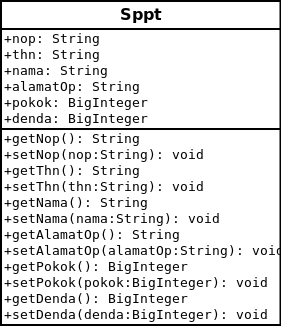
\includegraphics[width=0.5\textwidth]{./resources/uml/uml-class-Sppt}
  \caption{Diagram Kelas Sppt}
  \label{fig:uml-class-Sppt}
\end{figure}

Kelas Sppt ini terdiri dari 6 (enam) properti dan 12 (dua belas) \textit{method}. Enam properti ini adalah nilai-nilai yang dikembalikan dari hasil eksekusi \textit{store procedure} pada basis data. Properti pada kelas ini terdiri dari :

\begin{itemize}
\item nop. Properti ini untuk menyimpan Nomor Objek Pajak, sebagai identitas kunci, tiap objek pajak akan memiliki NOP yang berbeda-beda.
\item thn. Properti ini untuk menampung Tahun Pajak dimana objek pajak dimunculkan tagihan pajaknya.
\item nama. Properti ini akan menampung nama dari wajib pajak untuk nomor objek pajak tersebut pada properti nop.
\item alamatOp. Properti ini untuk menampung alamat dari objek pajak, yang nantinya bisa digunakan sebagai bahan verifikasi bahwa objek tersebut adalah benar yang akan dicari tahu informasinya.
\item pokok. Properti ini untuk menampung besarnya tagihan pokok atas nomor objek pajak yang tersebut pada properti nop.
\item denda. Properti ini akan menampung besarnya denda administrasi yang ditetapkan apabila ada keterlambatan pembayaran pajak yang telah melewati tanggal jatuh temponya.
\end{itemize}

Seluruh \textit{method} yang disediakan pada kelas ini hanya bertujuan untuk melakukan akses terhadap properti pada kelas ini.

\section{Kelas PembayaranSppt}

Kelas PembayaranSppt berfungsi untuk menampung informasi dari respon pencatatan pembayaran SPPT yang terjadi. Diagram kelas dari PembayaranSppt ini seperti terlihat pada gambar \ref{fig:uml-class-PembayaranSppt} :

\begin{figure}[H]
  \centering
  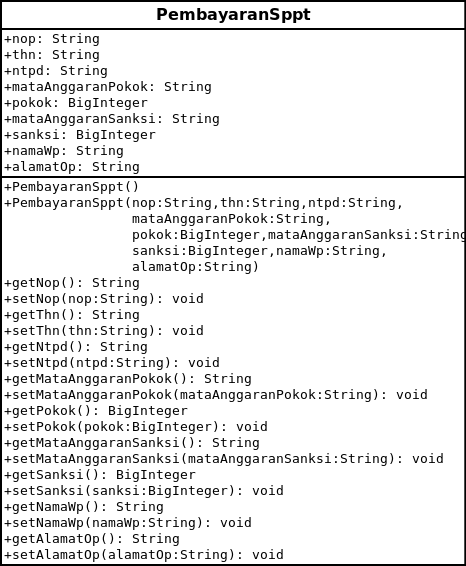
\includegraphics[width=0.5\textwidth]{./resources/uml/uml-class-PembayaranSppt}
  \caption{Diagram Kelas PembayaranSppt}
  \label{fig:uml-class-PembayaranSppt}
\end{figure}

Kelas ini memiliki 9 (sembilan) properti, 2 (dua) kontruktor, dan 18 (delapan belas) \textit{method}. Properti dari kelas ini terdiri dari :

\begin{itemize}
\item nop.
\item thn.
\item ntpd.
\item mataAnggaranPokok.
\item pokok.
\item mataAnggaranSanksi.
\item sanksi.
\item namaWp.
\item alamatOp.
\end{itemize}

\section{Kelas ReversalPembayaran}
\chapter{PERTIMBANGAN KHUSUS KINERJA SISTEM}

Sebagai bahan pertimbangan khusus agar sistem ini menjadi lebih sempurna, maka diperlukan kondisi jaringan yang aman. 

Maksudnya adalah, karena bentuk \textit{web services} REST dapat diakses oleh siapa pun dan dari mana pun, maka diperlukan filter keamanan pada sisi jaringan, artinya, hanya ada beberapa alamat IP saja yang dapat melakukan akses ke \textit{server web services} agar transaksi berjalan lebih aman.

Kondisi jalur jaringan internet pun diperlukan lebih dari 1 (satu) jalur. Hal ini untuk melakukan penjagaan jalur komunikasi apabila ada 1 \textit{line} terputus karena faktor diluar kewenangan administrator pada DPPK maka \textit{line} yang lain akan melakukan \textit{backup} koneksi. 
\chapter{HASIL PEMODELAN}

Hasil pemodelan dari sistem aplikasi yang akan dibangun, secara internal sebetulnya sudah dibahas pada bagian Arsitektur Sistem dan diperjelas dengan penjelasan pada bagian Deskripsi Sub Sistem. 

Secara tampilan tatap muka (\textit{interface}) tidak akan menghasilkan apa-apa selain model dari format \textit{request} yang akan menjadi 3 (tiga) bagian berikut :

\begin{enumerate}
  \item \texttt{pospbb/sppt/\{nop\}/\{thn\}}
  
  \textit{Request} ini digunakan untuk \textit{inquiry} data tagihan PBB-P2, dimana \texttt{nop} nantinya digantikan dengan nomor objek pajak PBB-P2 tanpa tanda baca, dan \texttt{thn} adalah tahun pajak dimana NOP tersebut akan dilihat informasinya.
  
  \item \texttt{pospbb/bayar/\{nop\}/\{thn\}/\{tglBayar\}/\{jamBayar\}}
  
  \textit{Request} ini digunakan untuk melakukan pencatatan pembayaran, dimana \texttt{nop} adalah Nomor Objek Pajak yang dibayarkan, \texttt{thn} adalah tahun pajak yang dibayarkan, \texttt{tglBayar} adalah tanggal terjadinya pembayaran dalam format DDMMYYYY dimana DD adalah 2 (dua) digit tanggal dalam satu bulan, MM adalah 2 (dua) digit bulan, dan YYYY adalah tahun. \texttt{jamBayar} adalah jam dibayarkannya PBB-P2 dengan format HH24MI, dengan HH24 dimaksudkan adalah 2 (dua) digit jam dengan format 24 jam, dan MI adalah menitnya.
  
  \item \texttt{pospbb/reversal/\{nop\}/\{thn\}/\{ntpd\}}
  
  \textit{Request} ini adalah \textit{request} untuk melakukan \textit{reversal} data pembayaran, dimana \texttt{nop} adalah Nomor Objek Pajak yang akan dilakukan \textit{reversal}, \texttt{thn} adalah Tahun pajak untuk NOP yang akan dilakukan \textit{reversal}, sedangkan \texttt{ntpd} adalah Nomor Transaksi Penerimaan Daerah sebagai identitas pencatatan pembayaran yang telah terjadi.
  
\end{enumerate}

Ini adalah format standar yang nantinya digunakan untuk berkomunikasi dengan \textit{client} dalam hal ini pihak Bank sebagai tempat pembayaran dalam hal pencatatan transaksi pembayaran. 
\chapter{BIAYA DAN JADWAL}

Biaya yang dibutuhkan untuk membangun sistem aplikasi ini secara pembangunan sistem tidak ada, tetapi ada faktor pendukung agar sistem dapat berkomunikasi dengan \textit{client} yaitu :

\begin{itemize}
  \item Adanya VPN Server yang dapat mengamankan lalu lintas data melalui jaringan internet yang sifatnya publik dengan spesifikasi RAM ... dan prosesor ... yang diharapkan dapat melayani permintaan VPN \textit{Client} yang semakin bertambah. Rentang harganya akan terlihat relatif dari kisaran .. sampai dengan ...
   
  \item Adanya jaringan internet, dalam hal ini \textit{bandwidth} yang mampu menangani transaksi ratusan, bahkan ribuan dalam waktu yang hampir bersamaan. Kondisi akses jaringan internet ini diusahakan yang berjenis \textit{dedicated} dimana perbandingan unduh dan unggah akan berada pada 1:1. Kisaran harga untuk layanan ini pun variatif dari harga ... sampai dengan ... yang biasanya bergantung pada besarnya \textit{bandwidth} yang dibutuhkan.
  
\end{itemize} 

\backmatter%%%%%%%%%%%%%%%%%%%%%%%%%%%%%%%%%%%%%%%%%%%%%%%%%%%%%%%
\printindex

%%%%%%%%%%%%%%%%%%%%%%%%%%%%%%%%%%%%%%%%%%%%%%%%%%%%%%%%%%%%%%%%%%%%%%

\end{document}





